\documentclass[a4paper,11pt]{article}

\usepackage[utf8]{inputenc}    % Pour que LaTeX comprenne les accents.
\usepackage{times}             % Police de caractères
\usepackage[english]{babel}     % Traitement du texte adapté aux règles typographiques
                               % de la langue donnée en option (e.g., pour l'espacement
                               % après les ponctuations
\usepackage[T1]{fontenc}
\usepackage{amsmath, amsthm, amssymb} 
\usepackage{dsfont}  % pour les indicatrices 
\usepackage{graphicx} 
\usepackage{textcomp}  
\usepackage{enumerate}                             
\sloppy              % Ne pas faire déborder les lignes dans la marge


\newtheorem{lemma}{Lemma}
\newtheorem{cons}{Corollary}
\newtheorem{theo}{Theorem}

\theoremstyle{definition}
\newtheorem{definition}{Definition}
\newtheorem{process}{Process}

\theoremstyle{remark}
\newtheorem{remark}{Remark}

\title{Throwing needles on a coloured plane.}
\author{Thomas Bourgeat \and Marc Heinrich \and Paul Melotti 
\and Jean-Marc Robert}

\begin{document}
\maketitle

\begin{abstract} Colour the euclidian plane with $k$ colours, and throw a needle
``randomly'' on it. You get a certain probablity that the endpoints fall on 
different colours. How can one make this probability maximal?
This problem is related to finite graphs having unit-lengthed edges, to provide 
some bounds on the optimal probability.\end{abstract}

\section{Introduction}
A well-known problem of geometric graph theory is the following: how many colors
are needed to color the plane so that no two points at unit distance are the 
same color? This is known as the Hadwiger-Nelson problem, and the answer to that
question is often refered as the \textit{chromatic number of the plane}. It 
seems the problem was first stated by Nelson in 1950, and first published by 
Gardner in \cite{gardner}.
For a nice review about this problem and close relatives, see Soifer's book
\cite{soifer}. This question is still very mysterious to that day, and all that 
is known for sure is that the chromatic number of the plane is at least 4 and at
most 7.

The questions presented here may be seen as a probabilistic version of this 
problem, since we don't try to make \textit{every} unit-lengthed segment 
bichromatic but only a large fraction of them.
\begin{definition}
A $k$-\textit{colouring} of the plane is a function from the euclidian 
plane~$\mathbb{R} ^2$ to the finite set $\{1, \dots , k \}$.

If $B_R$ denotes the euclidian ball of center O and radius $R$ in 
$\mathbb{R} ^2$, and $d$ is the usual euclidian distance, the set of
\textit{needles} inside $B_R$ is noted
\[N_R = \{(x,y) \in B_R ^2 \mid d(x,y)=1\}. \]

A $k$-colouring $c$ is said to be \textit{valid} if, for any $R>0$, the set
\[ E_R = \{(x,y) \in N_R \mid c(x) = c(y) \} \]
is measurable, and the ratio $\frac{\lambda (E_R)}{\lambda (N_R)}$ 
converges to a limit $p(c) \in [0,1]$ as $R$ tends to infinity, where $\lambda$ 
is the Lebesgue measure (on $\mathbb{R}^4$).
\end{definition}

For instance, a borelian periodic colouring is valid ; we will use this
particular case quite a lot.
%In that case $p(c)$ is
%an natural probability : if $c$ is $P$-periodic for a parallelogram $P$, throw one
%point uniformly on $P$ and choose the other endpoint uniformly on the circle of
%radius 1 around the firs point, using periodic border conditions when needed.
%Then one easil checks that the probability of getting a monochromatic needle is
%$p(c)$.
Throughout the article, we will always implicitely assume that our colourings be
valid. Our aim will be to make $p(c)$ as small as possible, since it is not hard
to make it big.

Some other defintions are needed in order to relate this problem to finite
graphs.
\begin{definition}
\ 
\begin{enumerate}[a)]
\item For a finite graph $G=(V,E)$ and a $k$-colouring $c$ of the vertices of $G$, 
let $M(c)$ be the number of monochromatic edges in $G$ couloured with $c$.
Then define:
\[m_k(G) = \min_{c \ k-\mathrm{colouring \ of} \ G} \frac{M(c)}{|E|}.\]
\item A finite graph is said to be a \emph{unit distance graph} if it has 
an embedding in $\mathbb{R}^2$ in which all edges have length $1$.
\end{enumerate}
\end{definition}
In section~\ref{equiv} we prove the following:
\begin{theo} \label{ineg}
Let $\mathcal{G}$ be the set of unit distance graphs and $\mathcal{C}_k$ the set 
of valid $k$-colourings of the plane, then
$$ \sup_{g \in \mathcal{G}} \ m_k(g) \leq \inf_{c \in \mathcal{C}_k} \ p(c) \leq \frac{1}{k}. $$
\end{theo}

The particular cases $k=2,3$ are discussed in section~\ref{appli}, as well as a 
simple consequence using a strong theorem of De Bruijn and Erd\H{o}s :
\begin{cons}\label{con}
If $\inf_{c \in \mathcal{C}_k} \ p(c) = 0$ then the chromatic number of the
plane is at most $k$.
\end{cons}
Finally, we study in section~\ref{ext} the case of higher dimensions, and the
case of a finite table instead of the whole plane.

\section{Process equivalence}
\label{equiv}
%In this definition, as in the whole paper, when no further precision 
%is given the words ``uniform'' and ``uniformly'' refer to the Lebesgue measure -
%except when we choose in a finite set, where they have their usual meaning.
\begin{process} \label{premier}
Consider the following random variables :
\begin{itemize}
  \item let $A$ (the lowest end of the needle) be a point chosen uniformly 
  in $\mathbf{P}$ ;
  \item let $\theta$ be an independent angle chosen uniformly in $[0;\pi[$ ;
  \item let $B$ (the highest end of the needle) be $A + e^{i \theta}$.
\end{itemize}
\end{process}

Note that $B$ may all outside of $\mathbf{P}$. In that case, $c(B)$ is 
defined using the periodicity of the colouring.
Our goal is to evaluate and minimize the probability that both ends have the 
same color.

We consider the following, second process that will be very useful in our 
proofs. The idea is to throw a unit distance graph on the 
plane, and then to choose a needle on that graph~:
\begin{process}
Given a unit distance graph $(G,V)$, represented in the plane in 
a unit distance way, label the edges with numbers from 
$1$ to $m$. Choose~: 
\begin{itemize}
\item one point $A_0$ uniformly on the initial parallelogram $\mathbf{P}$ for 
the origin of the graph ;
\item an independent angle $\theta$ uniformly in $[0;2\pi[$, to rotate the graph ;
\item an independent index $i$ in $[| 1;m|]$.
\end{itemize}
Then, rotate the graph by the angle $\theta$, translate it so that the origin 
falls on  $A_0$, and take the needle $(A',B')$ corresponding to the $i^{th}$ 
edge of the obtained graph.
\end{process}

\begin{lemma}\label{huitre}
Let $(A,B)$ be the needle obtained by the first process, and
$(A',B')$ the one obtained by the second process. Let $c_1$ and $c_2$ denote 
two colors, and $c$ a valid colouring. Then, we 
have~:\\
 $$\mathbb{P}(c(A) = c_1, c(B) = c_2) = \mathbb{P}(c(A') = c_1, c(B') = c_2) $$ \\
 In particular, the probability doesn't depend on the graph 
 chosen. For a graph with only two vertices, we exactly get the initial process.
\end{lemma}

\begin{proof}
Conventions : 
\begin{itemize}
\item we take a graph $G=(V,E)$, and let $m = |E|$ be the number of its edges.

\item as usual, $\mathbf{P}$ is the parallelogram obtained by the periodicity 
of the colouring.

\item $\mathcal{A}(\mathbf{P})$ is the area of the parallelogram.

\item $i \in [|1;m|]$ is the index of one of the edges of $G$.

\item $\theta_i$ denotes the angle made by a horizontal line and the $i^{th}$ 
edge of the graph. The 
complex coordinates of the vertices of the $i^{th}$ edges before 
rotation/translation are named $z_i $ and $z_i + e^{i.\theta_i}$.

\end{itemize}

We prove the lemma by the following series of equalities :

\begin{eqnarray*}
& & \mathbb{P}(c(A') = c_1, c(B') = c_2) \\
  &=& \frac{1}{m}\sum_{i=1}^{m} \mathbb{P}(c(A') = c_1, c(B') = c_2 | i)  \\
  &=& \frac{1}{m}\sum_{i=1}^{m}  \frac{1}{2\pi}\int_{\theta =0} ^{2\pi} \frac{1}{\mathcal{A}(\mathbf{P})}\int\int_{A_0 \in \mathbf{P}} \mathbb{P}(c(A') = c_1, c(B') = c_2 | i, \theta, A_0) d\theta dx dy \\  
  &=& \frac{1}{m 2\pi \mathcal{A}(\mathbf {P})}\sum_{i=1}^{m}\int_{\theta =0} ^{2\pi} \int\int_{A_0 \in \mathbf{P}} \mathds{1}(c(A_0 + z_i e^{i\theta}) = c_1, c(A_0 +z_i e^{i\theta} + e^{i (\theta + \theta_i)}) = c_2) d\theta dx dy \\  
    &=& \frac{1}{m 2\pi \mathcal{A}(\mathbf{P})}\sum_{i=1}^{m} \int_{\theta =0} ^{2\pi} \int\int_{A_0 \in \mathbf{P}} \mathds{1}(c(A_0) = c_1, c(A_0 + e^{i (\theta + \theta_i)}) = c_2 ) d\theta dx dy \hspace{1 cm} (*)\\ 
    &=& \frac{1}{m 2\pi \mathcal{A}(\mathbf{P})}\sum_{i=1}^{m} \int_{\theta =0} ^{2\pi} \int\int_{A_0 \in \mathbf{P}} \mathds{1}(c(A_0) = c_1, c(A_0 + e^{i \theta}) = c_2 ) d\theta dx dy \\ 
    &=& \frac{1}{2\pi \mathcal{A}(\mathbf{P})}\int_{\theta =0} ^{2\pi} \int\int_{A_0 \in \mathbf{P}} \mathds{1}(c(A_0) = c_1, c(A_0 + e^{i \theta}) = c_2 ) d\theta dx dy \\ 
\end{eqnarray*}
Which gives exactly the same probability as the first process (except that the 
angle is taken in $[0;2\pi[$ here, instead of $[0;\pi[$, but it doesn't make 
any difference when looking only at the colors).

Equality $(*)$ is justified by the periodicity of our colouring.
\end{proof}

\begin{proof}
Consider a graph $g$ coloured with $n$ colours. When one chooses a needle
randomly on this graph the probability that both ends have the same
colours is clearly greater than $c_n(g)$. Applying lemma \ref{huitre} with $g$, 
it follows from the description of the second process that the probability 
$p(c)$ for any colouring $c$ is greater than $c_n(g)$.
\end{proof}
We still don't know wether or not this is actually an equality. It is for 
$n=2$, as will be shown thereafter.

\section{Applications} \label{appli}
\subsection{2 colours}

With two colors, we consider a triangle as our graph. 
As there is always at least two vertices with the same color, it's clear that 
the probability that $c_2(g) = \frac{1}{3}$. Thanks to Corollary~\ref{ineg}, 
we know that $p(c) \geq \frac13$ for any valid $c$.

This bound is optimal. Indeed, consider the colouring in figure~\ref{color}, 
constructed with parallel strips of width 
$l = \frac {\sqrt3}{2}$, with the upper side opened and the lower side closed. 

\begin{figure}[h]
\center
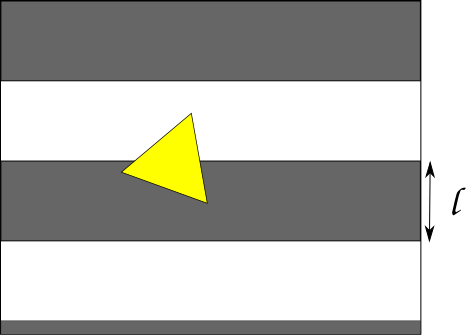
\includegraphics[scale=0.5]{path6509.png}
\caption{\label{couleur} The parallel stripes $2$-colouring}
\end{figure}

For this colouring, the probability of getting the same colour using the first 
process is $\frac13$. This can be shown by direct computation, or one can 
more simply remark that no unit-lengthed equilateral triangle can have its 
three vertices with the same colors. Applying Lemma~\ref{huitre}, we conclude 
that this colouring achieves a probability of $\frac{1}{3}$ indeed.
%CLASSE DE SOLUTIONS?

\subsection{3 colours}
 With three colors, we use the Moser spindle of Figure~\ref{color} - that 
 has at least one of its $11$ edges with both ends of the same colour.
 We similarly get that for $n=3$, the probability that both endpoints have the 
 same colour is at least 
 $\frac{1}{11}$ for any valid colouring. 

\begin{figure}[h]
\center
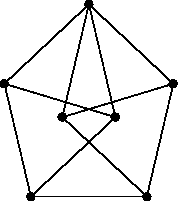
\includegraphics[scale=0.4]{T.png}
\caption{\label{color} The Moser spindle}
\end{figure}

We don't know if the previous bound is optimal. We believe that Figure~\ref{trois} 
can give a rather good $3$-colouring of the plane, for some well chosen length 
of the edge of the hexagons. Rough simulations have shown that this colouring gives a 
$p(c)$ of about $0.12$ for an edge of length about $0.61$. 
%Still, we did not compute the exact optimum in that case because the 
%estimation is still far away from $\frac{1}{11}$.

\begin{figure}[h]
\center
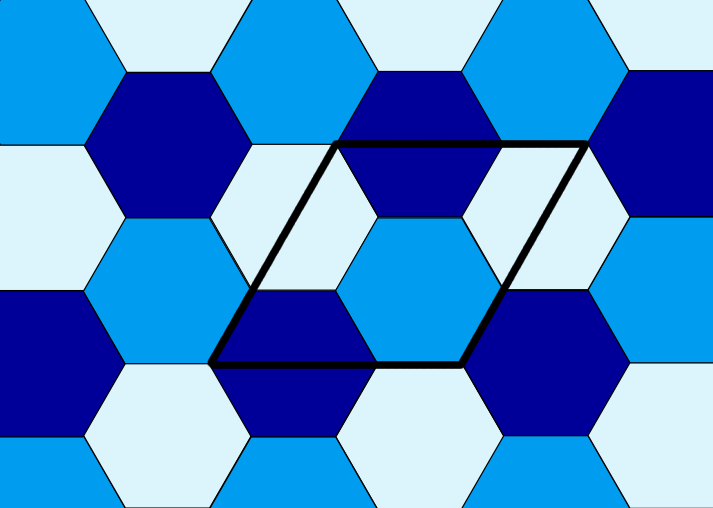
\includegraphics[scale=0.5]{trois.png}
\caption{\label{trois} A hexagonal $3$-colouring and its parallelogram of periodicity}
\end{figure}

\subsection{Connections with the Hadwiger-Nelson problem} \label{hn}
All results shown in this section will be derived using the axiom of choice. 
This is important to notice, since the answer to the Hadwiger-Nelson problem is 
suspected to depend on the set of axioms used. We will use the 
De Bruijn - Erd\H{o}s theorem, established in \cite{erdos}, whose proof uses 
the axiom of choice.
\begin{theo}[De Bruijn - Erdős]
 A graph $G$ can be coloured with $k$ colours iff all of its finite subgraphs 
 can be coloured with $k$ colours.
\end{theo}
In other words, the chromatic number of a graph is the maximum chromatic number 
of its finite subgraphs.

If there exist a unit distance graph (finite by definition) which cannot 
be coloured with $k$ colours, it 
follows from our study that the probability $p(c)$ for $c$ a periodic measurable 
$k$-colouring is always greater than a certain constant. Taking the 
contrapositive of this statement and using the De Bruijn-Erdős theorem, we get  
the interesting proposition :

Note that the final colouring of the plane we get is not necessarily periodic 
or even measurable, since its existence relies on a theorem that highly depends 
on the axiom of choice.

\section{Extensions}
\label{ext}
\subsection{Higher dimensions}
\label{dim}
The previous considerations can be extended to dimension $d \geq 3$, however, 
it becomes more complicated to write down. We have to consider a basis of 
vector leaving our colouring unchanged, and still denote by $\mathbf{P}$ the 
parallelepiped induced by these vectors.

The first process for choosing a needle now consist in~: 
\begin{itemize}
	\item choosing one point uniformly in the parallelepiped $ \mathbf{P} $ as 
	one point of the needle~;
	\item choosing independently one point uniformly on the unit sphere 
	$S^{d-1}$, uniformly to give the relative position of the second point.
\end{itemize}

Sending a unit-length graph on the $d$-dimensional space becomes somehow more 
complicated. We have to choose one initial point in $ \mathbf{P} $, and an independent 
rotation of the graph ; this can be achieved 
by using the Haar measure of $SO(d)$ uniformly. The second process now consists 
in : rotating the graph thanks to the matrix of $SO(d)$ chosen, translating it 
to the point of $\mathbf{P}$ chosen, and chosing one of the 
edges independently as your needle.

One can verify that the proof of Lemma~\ref{huitre} adapts to that definitions. 
It means that previous results still hold - namely, the probability that both 
ends fall on the same colour remains the same for the two processes. Crucial 
points of the proof are the invariance of the Haar measure under matrix product, and the 
fact that the image measure of said Haar measure by the application 
$M\mapsto Mv$, where $v$ is a given unit vector, is the uniform Lebesgue 
measure of $S^{d-1}$.

Thus, to find lower bonds on our probability, the same techniques may be applied 
in any finite dimension. For instance, in any dimension $d$ with $2$ colours,
the probability to get a monochromatic  
needle is always at least $\frac{1}{3}$ because of the equilateral triangle. 
We still don't know whether the bound of $\frac{1}{3}$ is achieved or not in 
dimension $3$ or more. 

Remark that in higher dimension, better minorants may be provided by 
Corollary~\ref{ineg}, since new graphs can 
become unit-length. For example, with $3$ colours in dimension $3$, the regular 
tetrahedron gives a better lower bound 
of $\frac 1 6 >\frac 1 {11}$. More generally, considering the complete graph 
$K_{k+1}$ in dimension $n$, which is unit distance and not $k$-colourable, the 
probability of getting a monochromatic needle is at least $\frac{1}{\binom{k+1}{2}}$ 
for $k$ colours in dimension $k$.

\subsection{Finite table}
\label{fini}

Previously we used periodicity so that we didn't have to worry about the second 
endpoint $B$ falling outside of $\mathbf{P}$, which made things much easier. We now 
try to require that $B$ fall in $\mathbf{P}$ to match a somewhat more practical 
view : we want to describe the throwing of the needle on an ``actual'' bounded 
table. The first difficulty is to find a natural distribution for our needle.

\begin{process} \label{encore}
Denote by $\mathbf{P}$ an open parallelogram, representing the table. For the 
process to be well defined, we need to assume that $\mathbf{P}$ can contain at
least one needle - equivalently, that $P(B \in \mathbf{P}) > 0$ since $\mathbf{P}$ 
is an open set.
\begin{itemize}
\item Consider the law of $(A,B)$ given by Pocess~\ref{premier}.
\item Take for your law the conditional probability given the event 
$\{B \in \mathbf{P} \}$.
\end{itemize}
\end{process}

To evaluate $P(B \in \mathbf{P})$ we need to define the border of a parallelogram~:
\begin{definition}
For $r>0$, let $K(\mathbf{P},r)$ the $r$-wide inner border of $\mathbf{P}$~:
\[K(\mathbf{P},r) = \{ z \in \mathbf{P} \mid d(z,\mathbf{P}^c) < r\} \] 
\end{definition}

\begin{figure}[h]
\center
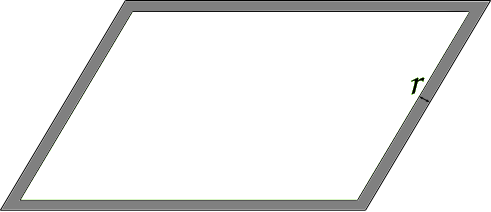
\includegraphics[scale=0.5]{tablefinie.png}
\caption{\label{tablefinie} The set $K(\mathbf{P},r)$ in grey}
\end{figure}

\begin{lemma}
Let $c$ be a $n$-colouring of $\mathbf{P}$. Denote by $p(c)$ the probability 
that both ends have the same colour when throwing 
the needle with Process~\ref{premier}, and $p'(c)$ for Process~\ref{encore}. Then 
there is a positive constant $\kappa \leq 2$ so that 
$$ | p'(c) - p(c)| \leq \kappa \frac{\mathcal{A}(K(\mathbf{P},1))}{\mathcal{A}(\mathbf{P})}.$$
\end{lemma}

\begin{proof}
We will show that the inequality is true for $\kappa =2$, but this is probably 
not the best constant.

Let $r = \frac{\mathcal{A}(K(\mathbf{P},1))}{\mathcal{A}(\mathbf{P})}$. When 
$r \geq \frac12$ the inequality is obvious, so we will now suppose that 
$r < \frac12$. Consider Process~\ref{premier} and denote by $\mathcal{M}$ the 
event ``both ends have same colours'', and by $\mathcal{N}$ the event ``$B$ 
falls inside of $\mathbf{P}$''. Then $P(\mathcal{N}^c) \leq r$, indeed, $B$ can 
be outside of $\mathbf{P}$ only
when $A$ is in $K(\mathbf{P},1)$. Easy computation shows that
\begin{eqnarray*}
p(c) - p'(c) & = & P(\mathcal{M}) - P(\mathcal{M} \mid \mathcal{N}) \\
& = & \frac{P(\mathcal{N}^c)}{P(\mathcal{N})} \left( P(\mathcal{M}\mid \mathcal{N}^c) - P(\mathcal{M})\right),
\end{eqnarray*}
and using the fact that $P(\mathcal{N}^c) \leq r$ and 
$P(\mathcal{N}) \geq 1-r \geq \frac12$ we get 
$$ |p(c) - p'(c)| \leq 2r.$$
\end{proof}

Since we already have bounds on $p$, we can therefore deduce bounds on $p'$.
For instance, with $2$ colours, we see that 
$p'(c) \geq \frac13 - \kappa \frac{\mathcal{A}(K(\mathbf{P},1))}{\mathcal{A}(\mathbf{P})}$. 
This bound becames sharper as the table parallelogram $\mathbf{P}$ becomes bigger.

%\section{Final notes}
%In the unbounded case, it may seem a bit disappointing that we chose to study 
%only periodic colourings. One can indeed hope for some similar results for a 
%larger class of colourings. For instance, one can think of the probability $p_R$ 
%of obtaining two same coloured endpoints when launching the needle on the square 
%$S(R)$ of side $R$ centered on $O$~: we could have said that a colouring is 
%\emph{valid} if $p_R$ converges 
%as $R \rightarrow \infty$. If we denote $p$ this limit, section~\ref{fini} 
%easily shows that all of the inequalities obtained are true for $p$. In 
%particular, Corollary~\ref{ineg} holds for this new definition when taking $C_n$ 
%the set of ``new'' valid colourings with $n$ colours, and Corollary~\ref{suite} 
%holds too for this class of colourings. 
%It's also clear that any periodic colouring is valid to that 
%definition. Still, we chose not to use that notion, because $p$ is not a 
%probability and shouldn't be 
%seen as such. It may though be the most natural way to give a sense to 
%the intuitive idea of ``throwing a needle uniformly on the whole plane''.

\subsection*{Acknowledgements}
We are very grateful to David Naccache for his constant help in the writing of
this paper, and to Eric Brier for many ideas and insight on the subject of 
unit distance graphs.

\bibliographystyle{abbrv}
\bibliography{Tiling}

\end{document}
